\chapter{Κύρια Αποτελέσματα} \label{Chapter2}

\section{Διατύπωση Προβλήματος} \label{Chapter2Section1}

\bigskip
Θεωρούμε το πρόβλημα Διμερούς Τηλεχειρισμού Ηγέτη-Ακόλουθου αποτελούμενο από δύο πανομοιότυπους ρομποτικούς βραχίονες με m αρθρώσεις, όπου ο Ηγέτης χειρίζεται από τον άνθρωπο. Τα συστήματά τους δίνονται από την δυναμική εξίσωση ενός βραχίονα:

\begin{equation}
  \mathbf{M}_{\kappa}(\mathbf{q}_\kappa) \ddot{\mathbf{q}}_\kappa + \mathbf{C}_{\kappa}(\mathbf{q}_\kappa, \dot{\mathbf{q}}_\kappa) \dot{\mathbf{q}}_\kappa + \mathbf{G}_{\kappa}(\mathbf{q}_{\kappa}) = \mathbf{u}_\kappa + \mathbf{\tau}_\kappa \label{robotic_manipulator_system}
\end{equation}

\noindent όπου
\begin{description}
  \item[\kappa:] Δείκτης με $\kappa = L$ για τον Ηγέτη και $\kappa = F$ για τον Ακόλουθο.
  \item[\mathbf{q}_{\kappa} \in \mathbb{R}^{m}:] Οι γωνίες των αρθρώσεων του ρομποτικού βραχίονα.
  \item[\mathbf{M}_{\kappa} \in \mathbb{R}^{m \times m}:] Ο θετικά ορισμένος και συμμετρικός πίνακας αδρανείας του βραχίονα.
  \item[\mathbf{C}_{\kappa} \in \mathbb{R}^{m \times m}:] Ο πίνακας Coriolis, κεντρομόλων δυνάμεων και δυνάμεων τριβών.
  \item[\mathbf{G}_{\kappa} \in \mathbb{R}^{m}:] Το διάνυσμα των βαρυτικών ροπών.
  \item[\mathbf{u}_{\kappa} \in \mathbb{R}^{m}:] Η είσοδος ελέγχου του συστήματος.
  \item[\mathbf{\tau}_{L} = \mathbf{\tau}_{h} \in \mathbb{R}^{m}:] Η εφαρμοσμένη ρόπη στον Ηγέτη μέσω της εξασκούμενης δύναμης από τον άνθρωπο.
  \item[\mathbf{\tau}_{F} = \mathbf{0}:] Η εφαρμοσμένη ροπή στον Ακόλουθου, καθώς θεωρούμε ότι δεν έρχεται σε επαφή με το περιβάλλον του.
\end{description}

\bigskip
Θεωρώντας τις καταστάσεις \( \mathbf{x}_{\kappa 1} = \mathbf{q}_{\kappa} \) και \( \mathbf{x}_{\kappa 2} = \dot{\mathbf{q}}_{\kappa} \), η εξίσωση (\bref{robotic_manipulator_system}) γράφεται ως:

\begin{align}
  \dot{\mathbf{x}}_{\kappa 1} & = \mathbf{x}_{\kappa_2} \label{xkappa1dot}                                                                                      \\
  \dot{\mathbf{x}}_{\kappa 2} & = \mathbf{f}_{\kappa}(\mathbf{x}_{\kappa 1}, \mathbf{x}_{\kappa 2}) + \mathbf{g}(\mathbf{x}_{\kappa 1})(\mathbf{\tau}_{\kappa} + \mathbf{u}_{\kappa}) \label{xkappa2dot}
\end{align}
όπου
\begin{align*}
  \mathbf{f}_{\kappa}(\mathbf{x}_{\kappa_1}, \mathbf{x}_{\kappa_2}) & = \mathbf{M}_{\kappa}^{-1}(\mathbf{x}_{\kappa_1}) \mathbf{C}_{\kappa}(\mathbf{x}_{\kappa_1}, \mathbf{x}_{\kappa_2}) \mathbf{x}_{\kappa_2} \in \mathbb{R}^{m} \\
  \mathbf{g}_{\kappa}(\mathbf{x}_{\kappa_1})               & = \mathbf{M}_{\kappa}^{-1}(\mathbf{x}_{\kappa_1}) > 0 \in \mathbb{R}^{m \times m}
\end{align*}
καθώς \( \mathbf{M}_{\kappa} \) είναι θετικά ορισμένος. Επιπλέον, λόγω των ιδιοτήτων των \( \mathbf{M}_{\kappa} \) και \( \mathbf{C}_{\kappa} \), οι συναρτήσεις \( \mathbf{f}_{\kappa} \) και \( \mathbf{g}_{\kappa} \) είναι τοπικά Lipschitz συναρτήση των \( \mathbf{x}_{\kappa_1},  \mathbf{x}_{\kappa_2} \).

\bigskip
Περαιτέρω, αναλύοντας τις εξισώσεις (\bref{xkappa1dot}), (\bref{xkappa2dot}) για κάθε άρθρωση \( i = 1, \dots, m \), παίρνουμε:
\begin{align}
  \dot{x}_{\kappa_{1,i}} & = x_{\kappa_{2,i}} \label{xkappa1dotwithi}                                                                                                         \\
  \dot{x}_{\kappa_{2,i}} & = f_{\kappa_i}(\mathbf{x}_{\kappa_1}, \mathbf{x}_{\kappa_2}) + \sum_{j=1}^{m} g_{\kappa_{i,j}}(\mathbf{x}_{\kappa_1})(\tau_{\kappa_j} + u_{\kappa_j}) \label{xkappa2dotwithi}
\end{align}
όπου \( \mathbf{x}_{\kappa_j} = [ x_{\kappa_{j,1}} \dots  x_{\kappa_{j,m}} ]^{T} \), \( j = 1, 2 \), είναι οι καταστάσεις του Ηγέτη και του Ακόλουθου, για \( \kappa \in \{ L, F \} \) αντίστοιχα, με \( x_{L_{1,i}} \), \( x_{F_{1,i}} \) και \( x_{L_{2,i}} \), \( x_{F_{2,i}} \), \( i = 1, \dots, m \), να αντιπροσωπεύουν τη γωνιακή θέση και ταχύτητα κάθε άρθρωσης. Επιπλέον, οι \( f_{\kappa_i} \), \( g_{\kappa_{i,j}} \), όπου \( i, j = 1, \dots, m \), \( \kappa \in \{ L, F \} \), δηλώνουν το \( i \)-οστό και το \( i,j \)-οστό στοιχείο των \( f_{\kappa} \) και \( g_{\kappa} \), και τα \( u_{\kappa_j} \), \( \tau_{\kappa_j} \), \( j = 1, \dots, m \), \( \kappa \in \{ L, F \} \), δηλώνουν το \( j \)-οστό στοιχείο των \( u_{\kappa} \) και \( \tau_{\kappa} \), αντίστοιχα.

Για το σύστημα (\bref{xkappa1dotwithi})-(\bref{xkappa2dotwithi}) πραγματοποιούνται οι εξής υποθέσεις:\\

\begin{hypothesis}\label{hyp:1}
Η ροπή που ασκεί ο άνθρωπος είναι ομοιόμορφα φραγμένη. Επομένως, υπάρχουν άγνωστες σταθερές $\bar{\tau}_{h_{i}}$, $i=1,...m$, τέτοια ώστε $\left|\tau_{h_{i}}(t)\right| \leq \bar{\tau}_{h_{i}}, \forall t \geq 0$.\\
\end{hypothesis}

\begin{hypothesis}\label{hyp:2}
Η λύση των διαφορικών εξισώσεων κατάστασης των συστημάτων υπάρχει, είναι φραγμένη, και θεωρείται γνωστή για σχεδιαστικό έλεγχο για κάθε $t\in[-T_{D}(t), 0]$.\\
\end{hypothesis}

\begin{hypothesis}\label{hyp:3}
Η καθυστέρηση στο κανάλι επικοινωνίας είναι συνεχής με άνω φράγμα $T_{D}(t) \leq \bar{T}_{D},\text{ }$ $\forall t\geq 0$ και παραγωγίσιμη με $\dot{T}_{D}(t) < 1,\text{ } \forall t \geq 0$ .\\
\end{hypothesis}

\begin{observation}\label{obs:1}
Η Υπόθεση~\bref{hyp:3} είναι καθοριστικής σημασίας για την ορθή αντιμετώπιση της άγνωστης και συνεχώς μεταβαλλόμενης χρονικής καθυστέρησης, καθώς η απαίτηση για άνω φραγμό της παραγώγου $\dot{T}_{D}(t) \leq 1$ εξασφαλίζει ότι η ταχύτητα μεταβολής της καθυστέρησης παραμένει εντός ελεγχόμενων ορίων. Αυτός ο περιορισμός είναι κρίσιμος, διότι αποτρέπει την εμφάνιση ανεξέλεγκτων διακυμάνσεων στη χρονική καθυστέρηση που θα μπορούσαν να διαταράξουν την αλληλουχία των δεδομένων στο σύστημα Ηγέτη-Ακόλουθου. Επιπλέον, η διατήρηση αυτής της συνθήκης διασφαλίζει την ικανοποίηση της αρχής \textbf{FIFO} (First-In/First-Out) \cite{bresch2018robust}, η οποία εγγυάται ότι τα δεδομένα που εισέρχονται πρώτα στο σύστημα τους καθενός ρομποτικού βραχίονα θα επεξεργαστούν και θα εξέρχονται επίσης πρώτα, αποτρέποντας τη δημιουργία ανακατανομής ή σύγχυσης στην ακολουθία τους. Αυτός ο φραγμός καθίσταται απαραίτητος για τη σταθερότητα και τη συνεπή λειτουργία του ελεγκτικού σχήματος, ειδικά σε συστήματα όπου οι χρονικές καθυστερήσεις είναι αβέβαιες και μεταβαλλόμενες.
\end{observation}

\begin{figure}[!ht]
  \begin{center}
    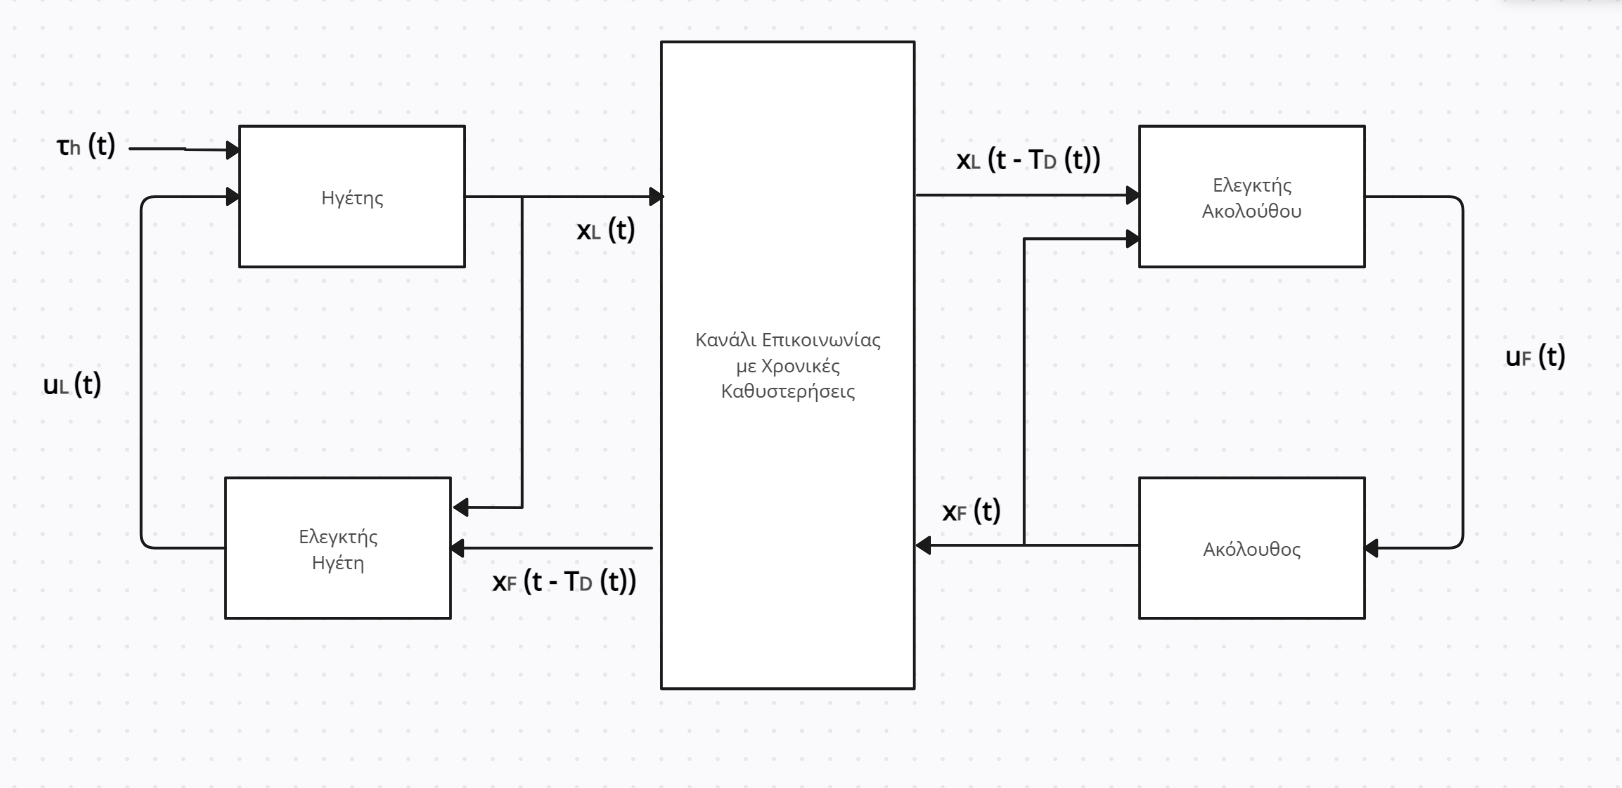
\includegraphics[width=1\linewidth]{Chapters/Chapter2/Figures/Control_System_Schema.png}
    \caption[Το κλειστό ΣΔΤΗΑ υπό εξέταση]{Το κλειστό ΣΔΤΗΑ υπό εξέταση}
    \label{system}
  \end{center}
\end{figure}

\section{Σχεδιασμός Ελέγχου} \label{Chapter2Section2}

\bigskip
Από τον Ορισμό~\bref{T_function_def} και για $L=U=1$, παίρνουμε την συνάρτηση μετασχηματισμού σφάλματος $T$:

\begin{equation}
  T : (-1, 1) \rightarrow \mathbb{R}, \quad T(\sigma) = \ln\left( \frac{1 + \sigma}{1 - \sigma} \right) \label{T_function_with_values}
\end{equation}
η οποία εξ ορισμού είναι γνησίως αύξουσα, άρα και ένα προς ένα. Επομένως, η αντίστροφη συνάρτηση \( T^{-1} \):

\begin{equation}
  T^{-1} : \mathbb{R} \rightarrow (-1, 1), \quad T^{-1}(\sigma) = \ln\left( \frac{\exp({\sigma}) - 1}{\exp({\sigma}) + 1} \right) \label{T_inv_function}
\end{equation}
αποδεικνύεται πως είναι επίσης αύξουσα και περιττή.

Για την σχεδίαση του ελεγκτή, κρίνεται απαραίτητο να παρατεθούν επιπλέον οι παρακάτω ορισμοί:
\bigskip
\begin{definition} \label{Sigma_function_def}
Για σταθερή σχεδιαστική παράμετρο \( \gamma \in (0, 1) \), η συνάρτηση \( S(\sigma; \gamma) \) ορίζεται ως:

\begin{equation}
  S(\sigma; \gamma) =
  \begin{cases}
    0,                                               & -\gamma \leq \sigma \leq \gamma \\[0.3cm]
    (\sigma - \operatorname{sign}(\sigma) \gamma)^2, & \gamma < |\sigma| < 1
  \end{cases} \nonumber
\end{equation}
Μπορούμε να γράψουμε:
\begin{equation}
  S(\sigma; \gamma) =
  \begin{cases}
    0,                   & -\gamma \leq \sigma \leq \gamma \\[0.3cm]
    (\sigma - \gamma)^2, & \gamma < \sigma < 1             \\[0.3cm]
    (\sigma + \gamma)^2, & -1 < \sigma < -\gamma
  \end{cases}\label{Sigma_function}
\end{equation}
\end{definition}

Έτσι, λοιπόν, από τις σχέσεις (\bref{T_function_with_values})-(\bref{Sigma_function}), προκύπτει η συνάρτηση:
\begin{equation*}
  S(\sigma; \gamma) \times T(\sigma) =
  \begin{cases}
    0,                                      & -\gamma \leq \sigma \leq \gamma \\[0.3cm]
    (\sigma - \gamma)^2 \ln\left( \frac{1 + \sigma}{1 - \sigma} \right), & \gamma < \sigma < 1 \\[0.3cm]
    (\sigma + \gamma)^2 \ln\left( \frac{1 + \sigma}{1 - \sigma} \right), & -1 < \sigma < -\gamma
  \end{cases}
\end{equation*}
η οποία είναι επίσης γνησίως αύξουσα.

\bigskip
\begin{definition} \label{B_function_def}
Oρίζεται η μερική παράγωγος \( B(\sigma) \):
\begin{equation}
  B(\sigma) = \frac{\partial T}{\partial \sigma} = \frac{2}{1 - \sigma^2}, \quad \sigma \in (-1, 1) \label{B_function}
\end{equation}
\end{definition}

\bigskip
\begin{definition} \label{Gamma_function_def}
Oρίζεται η μερική παράγωγος \( \Gamma(\sigma; \gamma) \):
\begin{equation}
  \Gamma(\sigma; \gamma) = \frac{\partial [S T]}{\partial \sigma} =
  \begin{cases}
    0,                                                                                                                                                               & -\gamma \leq \sigma \leq \gamma \\[0.3cm]
    \displaystyle \frac{2(\sigma - \gamma)\left[ (\sigma^2 - 1)\ln\left( \frac{\sigma + 1}{1 - \sigma} \right) - \sigma + \gamma \right]}{(\sigma - 1)(\sigma + 1)}, & \gamma < \sigma < 1             \\[0.5cm]
    \displaystyle \frac{2(\sigma + \gamma)\left[ (\sigma^2 - 1)\ln\left( \frac{\sigma + 1}{1 - \sigma} \right) - \sigma - \gamma \right]}{(\sigma - 1)(\sigma + 1)}, & -1 < \sigma < -\gamma
  \end{cases} \label{Gamma_function}
\end{equation}
\end{definition}

\bigskip
Στο παρακάτω σχήμα (\bref{fig:functions_plots}) απεικονίζονται οι προαναφερθέντες συναρτήσεις $T$ και $ST$, οι οποίες θα χρησιμοποιηθούν στον σχεδιαστικό μας έλεγχο παράλληλα με τις παραγώγους τους $B$ και $\Gamma$:

\begin{figure}[!ht]
	\centering
		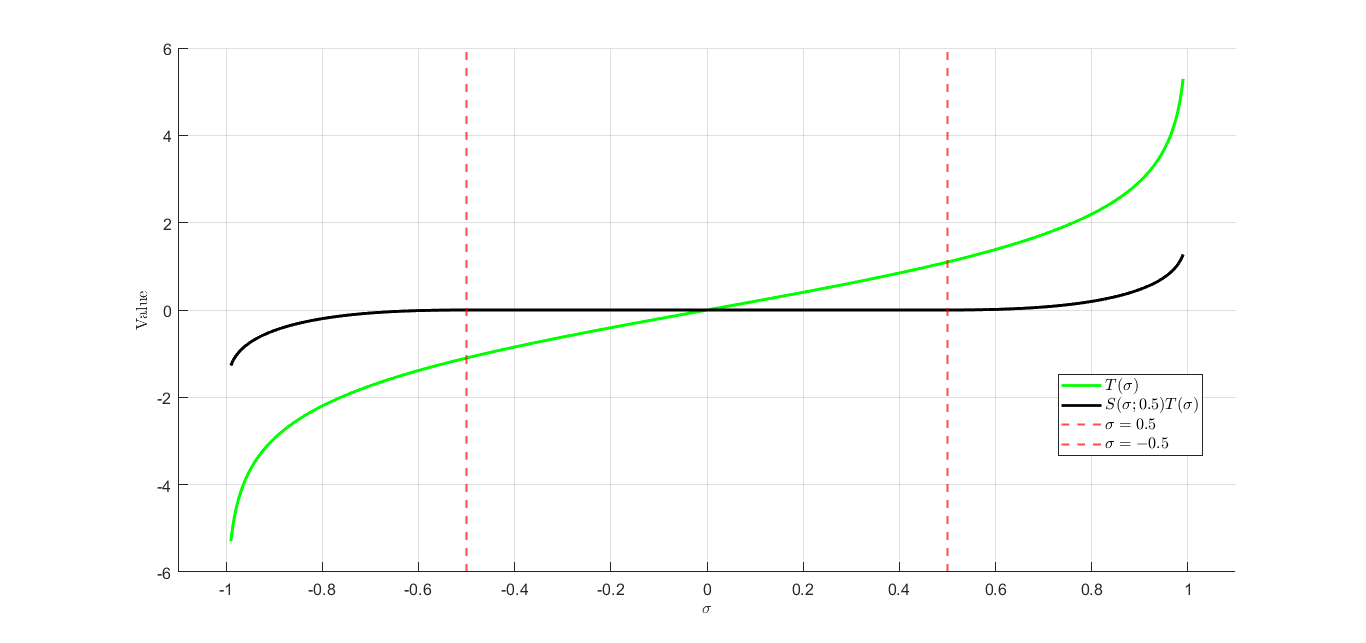
\includegraphics[width=1\linewidth]{Chapters/Chapter2/Figures/functions_plots.png}
	\caption[Γραφική Παράσταση των συναρτήσεων $T$ και $ST$]{Γραφική Παράσταση των συναρτήσεων $T$ και $ST$}
	\label{fig:functions_plots}
\end{figure}

\bigskip
Ο σχεδιαστικός έλεγχος που ακολουθεί είναι βασισμένος σε αυτόν που προτάθηκε στην \cite{BIKAS20239972}, με τις απαραίτητες διαφοροποιήσεις και προσθήκες για την επίτευξη των δύο στόχων που παρατέθηκαν στην Ενότητα~\bref{Chapter1Section3}. Παρατίθονται μερικοί ορισμοί χρήσιμοι για την κατανόηση του σχεδιαστικού ελέγχου:
\begin{itemize}
  \item $t_1$: η στιγμή κατά την οποία ο Ακόλουθος εισέρχεται στην Περιοχή Κινδύνου Ακόλουθου(\textbf{ΠΚΑ}), (βλέπε αρχή Ενότητας~\bref{Chapter2Section3}),
  \item $Q_{S_{i}}$: το διαχωριστικό σύνορο ανάμεσα στις Περιοχή Ασφαλείας Ακόλουθου(\textbf{ΠΑΑ}) και Περιοχή Κινδύνου Ακόλουθου(\textbf{ΠΚΑ}) για κάθε γωνία,
  \item $Q_{F_{i}}$: ο περιορισμός εξόδου του Ακόλουθου για κάθε γωνία
\end{itemize}

\bigskip
Επιπλέον, στο Σχήμα~\bref{control_concept}, για να δωθεί μια διαισθητική κατανόηση της επιδιωκώμενης συμπεριφοράς του σχεδιαστικού ελέγχου για την αποφυγή των περιορισμών, παρουσιάζονται οι δύο διακριτές περιοχές λειτουργίας του Ακόλουθου: η Περιοχή Ασφαλείας Ακόλουθου(\textbf{ΠΑΑ}) και η Περιοχή Κινδύνου Ακόλουθου(\textbf{ΠΚΑ}). Σε αυτές τις περιοχές, η προτεραιότητα ελέγχου μεταβάλλεται ανάλογα με τον κίνδυνο που αντιμετωπίζει ο Ακόλουθος.

\begin{figure}[!ht]
  \begin{center}
    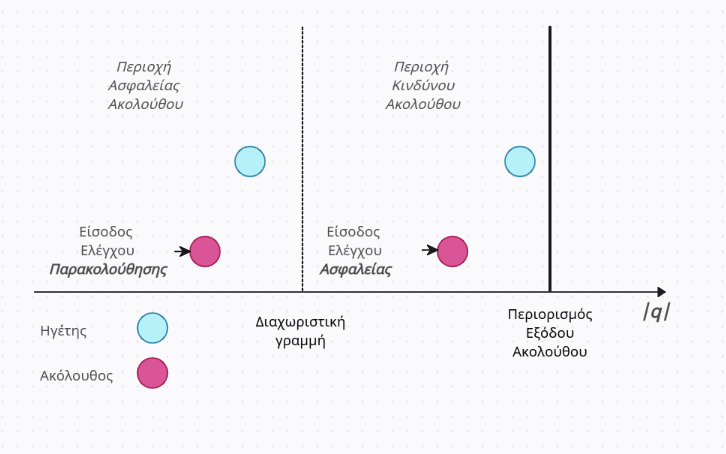
\includegraphics[width=1\linewidth]{Chapters/Chapter2/Figures/Control_Concept.png}
    \caption[Απεικόνιση στρατηγικής ελέγχου αλλαγής προτεραιότητας στο σύστημα του Ακόλουθου]{Απεικόνιση στρατηγικής ελέγχου αλλαγής προτεραιότητας στο σύστημα του Ακόλουθου}
    \label{control_concept}
  \end{center}
\end{figure}

\bigskip 
Παρακάτω παρατίθεται ο πλήρης σχεδιαστικός έλεγχος:

\begin{step}\label{step:1:control}
(για \( i = 1, \dots, m \)):
\bigskip
Κανονικοποιημένα σφάλματα
\begin{align}
  \xi_{L_{1,i}}(t) & = \frac{x_{L_{1,i}}(t) - x_{L_{1,i}}(0)}{\rho_{L_{1,i}}} \label{xiL1}             \\[0.3cm]
  \xi_{F_{1,i}}(t) & = \frac{x_{F_{1,i}}(t) - x_{L_{1,i}}(t - T_D(t))}{\phi_{F_{1,i}}(t)} \label{xiF1} \\[0.3cm]
  \xi_{O_{1,i}}(t) & =
  \begin{cases}
    0,                                                                                                     & \text{αν } | x_{F_{1,i}}(t) | < Q_{S_i}                  \\[0.3cm]
    \operatorname{sign}(x_{F_{1,i}}(t)) \cdot \dfrac{| x_{F_{1,i}}(t) | - Q_{S_i}}{Q_{F_{1,i}} - Q_{S_i}}, & \text{αν } Q_{S_i} \leq | x_{F_{1,i}}(t) | < Q_{F_{1,i}}
  \end{cases} \label{xiO1}
\end{align}
όπου
\begin{align}
  \rho_{L_{1,i}} &> 0 \quad (\text{σταθερά}) \label{rhoL1_define} \\[0.3cm]
  \phi_{F_{1,i}}(t) &= \rho_{F_{1,i}}(t) + \zeta_{F_{1,i}}(t) \label{phiF1_define} \\[0.3cm]
  \rho_{F_{1,i}}(t) &= \left( \rho^{0}_{F_{1,i}} - \rho^{\infty}_{F_{1,i}} \right) e^{-\lambda_i t} + \rho^{\infty}_{F_{1,i}} \label{rhoF1_define} \\[0.3cm]
  \zeta_{F_{1,i}}(t) &=
  \begin{cases}
    0,                                                                       & \text{αν } | x_{F_{1,i}}(t) | < Q_{S_i}                  \\[0.3cm]
    k_{\zeta_{1,i}} \left| x_{F_{1,i}}(t) - x_{L_{1,i}}(t - T_D(t)) \right|, & \text{αν } Q_{S_i} \leq | x_{F_{1,i}}(t) | < Q_{F_{1,i}}
  \end{cases} \label{zetaF1_define}
\end{align}
με
\begin{align}
  \rho^{0}_{F_{1,i}}      & > \left| x_{F_{1,i}}(0) - x_{L_{1,i}}(-T_D(0)) \right| \label{rhoF10>} \\[0.3cm]
  \rho^{\infty}_{F_{1,i}} & > 0   \label{rhoinfty}              \\[0.3cm]
  \lambda_{i}        & > 0    \label{lambda}              \\[0.3cm]
  k_{\zeta_{1,i}}         & > 1    \label{kzeta1}              \\[0.3cm]
  0 < Q_{S_i}             & < Q_{F_{1,i}}\ \label{QsQF1}
\end{align}

\bigskip
Ενδιάμεσα σήματα ελέγχου
\begin{align}
  e_{L_{1,i}}(t) & = S\left( \xi_{L_{1,i}}(t); \gamma_{L_{1}} \right) T\left( \xi_{L_{1,i}}(t) \right) \label{eL1} \\[0.3cm]
  e_{F_{1,i}}(t) & = T\left( \xi_{F_{1,i}}(t) \right) \label{eF1}                                                  \\[0.3cm]
  e_{O_{1,i}}(t) & =
  \begin{cases}
    0,                                & \text{αν } | x_{F_{1,i}}(t) | < Q_{S_i}                  \\[0.3cm]
    T\left( \xi_{O_{1,i}}(t) \right), & \text{αν } Q_{S_i} \leq | x_{F_{1,i}}(t) | < Q_{F_{1,i}}
  \end{cases} \label{eO1}
\end{align}
και
\begin{align}
  \alpha_{L_{1,i}}(t) & = -k_{L_{1,i}} e_{L_{1,i}}(t) \label{alphaL1} \\[0.3cm]
  \alpha_{F_{1,i}}(t) & = -k_{F_{1,i}} e_{F_{1,i}}(t) \label{alphaF1} \\[0.3cm]
  \alpha_{O_{1,i}}(t) & =
  \begin{cases}
    0,                            & \text{αν } | x_{F_{1,i}}(t) | < Q_{S_i}                  \\[0.3cm]
    - k_{O_{1,i}} e_{O_{1,i}}(t), & \text{αν } Q_{S_i} \leq | x_{F_{1,i}}(t) | < Q_{F_{1,i}}
  \end{cases} \label{alphaO1}
\end{align}
με
\begin{gather}
  \gamma_{L_{1}} \in (0, 1), \label{gamma1} \\
  k_{L_{1,i}},\ k_{F_{1,i}},\ k_{O_{1,i}} > 0 \label{kappa1}
\end{gather}
\end{step}

\bigskip
\begin{step}\label{step:2:control}
(για \( i = 1, \dots, m \)):

\bigskip
Κανονικοποιημένα σφάλματα 
\begin{align}
  \xi_{L_{2,i}}(t) & = \frac{x_{L_{2,i}}(t) - \alpha_{L_{1,i}}(t)}{\rho_{L_{2,i}}} \label{xiL2}    \\[0.3cm]
  \xi_{F_{2,i}}(t) & = \frac{x_{F_{2,i}}(t) - \alpha_{F_{1,i}}(t)}{\phi_{F_{2,i}}(t)} \label{xiF2} \\[0.3cm]
  \xi_{O_{2,i}}(t) & =
  \begin{cases}
    0,                                                         & \text{αν } | x_{F_{1,i}}(t) | < Q_{S_i}                  \\[0.3cm]
    \dfrac{x_{F_{2,i}}(t) - \alpha_{O_{1,i}}(t)}{Q_{F_{2,i}}}, & \text{αν } Q_{S_i} \leq | x_{F_{1,i}}(t) | < Q_{F_{1,i}}
  \end{cases} \label{xiO2}
\end{align}
όπου οι σταθερές ικανοποιούν
\begin{align}
  \rho_{L_{2,i}}     & > \left| x_{L_{2,i}}(0) \right| \label{rhoL2_define}                                                                                                                                                                     \\[0.3cm]
  \phi_{F_{2,i}}(t)  & = \rho_{F_{2,i}} + \zeta_{F_{2,i}}(t) \label{phiF2_define}                                                                                                                                                               \\[0.3cm]
  \rho_{F_{2,i}}     & > \left| x_{F_{2,i}}(0) - \alpha_{F_{1,i}}(0) \right| \label{rhoF2_define}                                                                                                                                               \\[0.3cm]
  \zeta_{F_{2,i}}(t) & =
  \begin{cases}
    0,                                                                   & \text{αν } | x_{F_{1,i}}(t) | < Q_{S_i}                  \\[0.3cm]
    k_{\zeta_{2,i}} \left| x_{F_{2,i}}(t) - \alpha_{F_{1,i}}(t) \right|, & \text{αν } Q_{S_i} \leq | x_{F_{1,i}}(t) | < Q_{F_{1,i}}
  \end{cases} \label{zetaF2_define}\\[0.3cm]
  k_{\zeta_{2,i}}    & > 1 \label{kzeta2}                                                                                                                                                                                                              \\[0.3cm]
  Q_{F_{2,i}}        & > \left| x_{F_{2,i}}(t_1) - \alpha_{O_{1,i}}(t_1) \right| \label{QF2}
\end{align}

\bigskip
Ενδιάμεσα σφάλματα ελέγχου:
\begin{align}
  e_{L_{2,i}}(t) & = S\left( \xi_{L_{2,i}}(t); \gamma_{L_{2}} \right) T\left( \xi_{L_{2,i}}(t) \right) \label{eL2} \\[0.3cm]
  e_{F_{2,i}}(t) & = T\left( \xi_{F_{2,i}}(t) \right) \label{eF2}                                                  \\[0.3cm]
  e_{O_{2,i}}(t) & =
  \begin{cases}
    0,                                & \text{αν } | x_{F_{1,i}}(t) | < Q_{S_i}                  \\[0.3cm]
    T\left( \xi_{O_{2,i}}(t) \right), & \text{αν } Q_{S_i} \leq | x_{F_{1,i}}(t) | < Q_{F_{1,i}}
  \end{cases} \label{eO2}
\end{align}
και
\begin{align}
  \alpha_{L_{2,i}}(t) & = -k_{L_{2,i}} \cdot \frac{\Gamma\left( \xi_{L_{2,i}}(t); \gamma_{L_{2}} \right)}{\rho_{L_{2,i}}} \cdot e_{L_{2,i}}(t) \label{alphaL2} \\[0.3cm]
  \alpha_{F_{2,i}}(t) & = -k_{F_{2,i}} \cdot \frac{B\left( \xi_{F_{2,i}}(t) \right)}{\phi_{F_{2,i}}(t)} \cdot e_{F_{2,i}}(t) \label{alphaF2}                   \\[0.3cm]
  \alpha_{O_{2,i}}(t) & =
  \begin{cases}
    0,                                                                                             & \text{αν } | x_{F_{1,i}}(t) | < Q_{S_i}                  \\[0.3cm]
    - k_{O_{2,i}} \cdot \dfrac{B\left( \xi_{O_{2,i}}(t) \right)}{Q_{F_{2,i}}} \cdot e_{O_{2,i}}(t), & \text{αν } Q_{S_i} \leq | x_{F_{1,i}}(t) | < Q_{F_{1,i}}
  \end{cases} \label{alphaO2}
\end{align}
όπου
\begin{gather}
  \gamma_{L_{2}} \in (0, 1), \label{gamma2} \\
  k_{L_{2,i}},\ k_{F_{2,i}},\ k_{O_{2,i}} > 0 \label{kappa2}
\end{gather}

\bigskip
Τελικά, σχεδιάζουμε τις εισόδους ελέγχου για το σύστημα ως εξής:
\begin{align}
  u_{L_{i}}(t) & = \alpha_{L_{2,i}}(t) + u_{H_{i}}(t) \label{uL} \\[0.3cm]
  u_{F_{i}}(t) & =
  \begin{cases}
    \alpha_{F_{2,i}}(t),                       & \text{αν } | x_{F_{1,i}}(t) | < Q_{S_i}                  \\[0.3cm]
    \alpha_{F_{2,i}}(t) + \alpha_{O_{2,i}}(t), & \text{αν } Q_{S_i} \leq | x_{F_{1,i}}(t) | < Q_{F_{1,i}}
  \end{cases} \label{uF}
\end{align}
όπου
\begin{equation}
  u_{H_{i}}(t) = -k_{H_{i}} \left( x_{L_{1,i}}(t) - x_{F_{1,i}}(t - T_D(t)) \right), \quad k_{H_{i}} > 0 \label{uH}
\end{equation}
\end{step}

\bigskip
\begin{observation} \label{obs:control:1}
Ο έλεγχος του Ηγέτη παραμένει αμετάβλητος καθ’ όλη τη διάρκεια, όπως ορίζεται στην \cite{BIKAS20239972}. Ωστόσο, ο έλεγχος του Ακόλουθου διαχωρίζεται σε δύο διακριτές περιοχές: την \textbf{Περιοχή Ασφαλείας Ακόλουθου (ΠΑΑ)}, όταν $|x_{F_{1, i}}(t)| < Q_{S_{i}}$, και την \textbf{Περιοχή Κινδύνου Ακόλουθου (ΠΚΑ)}, όταν $Q_{S_{i}} \leq |x_{F_{1, i}}(t)| < Q_{F_{i}}$. Στην ΠΑΑ, ο έλεγχος παραμένει ίδιος με αυτόν που περιγράφεται στη \cite{BIKAS20239972}, με αποκλειστικό στόχο την πιστή αναπαράσταση της καθυστερημένης τροχιάς του Ηγέτη. Αντίθετα, στην ΠΚΑ, οι συναρτήσεις επίδοσης προσαρμόζονται μέσω της προσθήκης σημάτων $\zeta_{F_{j, i}} \geq 0, j=1,2, i=1,...,m$, τα οποία εξαρτώνται από τα σφάλματα παρακολούθησης. Καθώς ο Ακόλουθος εισέρχεται στην ΠΚΑ, μειώνεται η προτεραιότητα στην ακριβή παρακολούθηση της τροχιάς του Ηγέτη, ενώ αυξάνεται η προτεραιότητα στην αποφυγή του περιορισμού κατάστασης στη θέση $Q_{F_{i}}$, όπως εκφράζεται από τα σήματα με δείκτη \textbf{O}. Οι δύο αυτοί στόχοι ελέγχου εξισορροπούνται στο σήμα εισόδου ελέγχου του Ακόλουθου (\ref{uF}) εντός της \textbf{ΠΚΑ} και πριν από τον περιορισμό, καθώς ο Ηγέτης συνεχίζει την πορεία του πέρα από αυτή τη θέση, με τον Χειριστή να αισθάνεται την ποιότητα της παρακολούθησης μέσω της απτικής ανάδρασης.
\end{observation}

\begin{observation} \label{obs:control:2}
Στην (\bref{QF2}), ο υπολογισμός της σταθεράς $Q_{F_{2}}$ πραγματοποείται την χρονική στιγμή εισαγωγής στην ΠΚΑ $t_1$, πράγμα που σημαίνει ότι επιβάλλεται να υπολογιστεί κατά την εξέλιξη του ελέγχου και όχι προκαταβολικά.
\end{observation}

\begin{observation} \label{obs:control:3}
Τα σταθερά κέρδη (\bref{kzeta1}), (\bref{kzeta2}) επιλέγονται > 1, έτσι ώστε στην ΠΚΑ, τα κανονικοποιημένα σφάλματα στον Ακόλουθο (\bref{xiF1}), (\bref{xiF2}), εξαιτίας των τροποποιημένων συναρτήσεων επίδοσης (\bref{phiF1_define}), (\bref{phiF2_define}),  να είναι καθαρά $\in(-1, 1)$, εξασφαλίζοντας την ευστάθεια τους εντός της ΠΚΑ.
\end{observation}

\begin{observation} \label{obs:control:4}
Ο ελεγκτής (\bref{xiF1})-(\bref{uH}) που προτάσσεται, όπως αναφέρθηκε και στην Ενότητα~\bref{Chapter1Section3}, είναι ανεξάρτητος από το μοντέλο του συστήματος του ρομποτικού βραχίονα, καθώς δεν απαιτεί καμία γνώση σχετικά με τη δυναμική του συστήματος Ηγέτη-Ακόλουθου. Επίσης, δεν εμπλέκει προσεγγιστικές δομές ή προσαρμοστικές τεχνικές για την απόκτηση αυτής της γνώσης, με αποτέλεσμα να προσφέρει μια λύση ελέγχου χαμηλής πολυπλοκότητας.
\end{observation}

\section{Ανάλυση Ευστάθειας} \label{Chapter2Section3}

\bigskip
\begin{theorem}\label{the:main}
Για το σύστημα (\bref{xkappa1dotwithi})-(\bref{xkappa2dotwithi}) και τις υποθέσεις (\bref{hyp:1})-(\bref{hyp:3}), ο σχεδιαστικός έλεγχος που αναπτύχθηκε στην Ενότητα~\bref{Chapter2Section2} εγγυάται, υπό την παρουσία μιας \textbf{άγνωστης, χρονικά μεταβαλλόμενης και συνεχούς καθυστέρησης στο κανάλι επικοινωνίας με γνωστό άνω φράγμα} $T_D(t) < \bar{T}_{D}, \quad \forall t>0$ και ενός περιορίσμου εξόδου στον Ακόλουθο, ότι:
Για κάθε $i = 1, \dots, m$, ισχύουν τα εξής:
\begin{enumerate}
    \item Τα σφάλματα $x_{F_{1,i}}(t) - x_{L_{1,i}}(t)$ συγκλίνουν στο σύνολο $( -\phi_{F_{1,i}}(t) - 2\rho_{L_{2,i}}\bar{T}_D$,  $\phi_{F_{1,i}}(t) + 2\rho_{L_{2,i}}\bar{T}_D )$.
    \item Όλα τα σήματα στο κλειστό βρόχο του συστήματος Ηγέτη-Ακόλουθου παραμένουν φραγμένα.
    \item Ισχύει ότι $|x_{F_{1,i}}(t)| < Q_{F_{1,i}}$, δηλαδή ο Ακόλουθος δεν θα έρθει σε επαφή με τον περιορισμό εξόδου.
\end{enumerate}
\end{theorem}

\bigskip
\begin{proof_of_theorem}\label{proof_of_the:main}

\bigskip
Αρχικά, θεωρούμε, χωρίς βλάβη της γενικότητας, ότι ο Ακόλουθος την χρονική στιγμή $t_1$ εισέρχεται στην περιοχή, δηλαδή την στιγμή κατά την οποία $|x_{F_{1, i}}(t)| = Q_{S_{i}}$. Όσο αφορά την περιοχή $|x_{F_{1, i}}(t)| < Q_{S_{i}}$, ο σχεδιαστικός έλεγχος παραμένει ο ίδιος με αυτόν που προτάθηκε στο (\cite{BIKAS20239972}), εξού και η ανάλυση ευστάθειας.
Θα αποδείξουμε ότι τα σφάλματα $e_{F_{j,i}}(t), e_{O_{j,i}}(t)$ θα είναι φραγμένα στο διάστημα $[t_1, +\infty)$. Από τις ιδιότητες της συνάρτησης (\bref{T_function_with_values}), οδηγούμαστε στο συμπέρασμα ότι
\begin{align*}
\left|\xi_{F_{j,i}}(t)\right|<1, \quad \left|\xi_{O_{j,i}}(t)\right|<1,
\end{align*}
το οποίο σημαίνει ότι όλα τα σφάλματα εξελίσσονται αυστηρά εντός των κατασκευασμένων καμπυλών επίδοσης.

\bigskip
Καθώς ο έλεγχος για τον Ηγέτη δεν έχει διαφοροποιηθεί από τον έλεγχο που προτάθηκε στο \cite{BIKAS20239972} στο $Q_{S_{i}} \leq |x_{F_{1, i}}(t)| < Q_{F_{1, i}}$ , συμπεραίνουμε	ότι τα σφάλματα $e_{L_{j,i}}(t)$ παραμένουν φραγμένα στο $t \in[t_1, \infty)$,και έτσι έχουμε
\begin{align*}
\left| \xi_{L_{j,i}}(t) \right| < 1, \quad \forall t\in[t_1, +\infty)
\end{align*}
και τις αντίστοιχες παρατηρήσεις και συμπεράσματα
\begin{align}
|x_{L_{1,i}}(t) - x_{L_{1,i}}(0)| &< \rho_{L_{1,i}} \label{conclusionL1} \\
|x_{L_{2,i}}(t) - \alpha_{L_{1,i}}(t)| &< \rho_{L_{2,i}} \label{conclusionL2}
\end{align}

\bigskip
Παίρνοντας την χρονική παράγωγο των παραπάνω κανονικοποιημένων σφαλμάτων από τις (\bref{xiF1}), (\bref{xiO1}), (\bref{xiF2}) και (\bref{xiO2}), θα έχουμε:
\begin{align}
\dot{\xi}_{F_{1, i}} &= \frac{1}{\phi_{F_{1,i}}}\left(\xi_{F_{2,i}}\phi_{F_{2,i}} - x_{L_{2,i}}(t-T_D(t))(1-\dot{T}_{D}(t)) - \xi_{F_{1,i}}\dot{\phi}_{F_{1,i}} + \alpha_{F_{1,i}}\right) \label{dotxiF1} \\
\dot{\xi}_{O_{1, i}} &= \frac{1}{Q_{F_{1, i}} - Q_{S_{i}}}\left(\xi_{O_{2, i}}Q_{F_{2, i}} + \alpha_{O_{1, i}}\right) \label{dotxiO1} \\
\dot{\xi}_{F_{2, i}} &= \frac{1}{\rho_{F_{2,i}}}\left(f_{F_{i}} - \dot{\alpha}_{F_{1,i}} - \xi_{F_{2, i}}\dot{\phi}_{F_{2, i}} + \sum_{j=1}^{m}g_{F_{i,j}}u_{F_{i}}\right) \label{dotxiF2} \\
\dot{\xi}_{O_{2, i}} &= \frac{1}{Q_{F_{2,i}}}\left(f_{F_{i}} - \dot{\alpha}_{O_{1,i}} + \sum_{j=1}^{m}g_{F_{i,j}}u_{F_{i}}\right) \label{dotxiO2}
\end{align}

\bigskip
Ορίζουμε το μη-κενό και ανοικτό σύνολο $\Omega_{\xi} = (-1,1) \subset \mathbb{R}$. Έχουμε από την (\bref{xiF1}) ότι
\begin{align}
\xi_{F_{1, i}}(t_{1}) &= \frac{x_{F_{1,i}}(t_1) - x_{L_{1,i}}(t_1 - T_D(t_1))}{\phi_{F_{1,i}}(t_1)} \nonumber \\
&= \frac{x_{F_{1,i}}(t_1) - x_{L_{1,i}}(t_1 - T_D(t_1))}{\rho_{F_{1, i}}(t_1) + k_{\zeta_{1, i}}|x_{F_{1,i}}(t_1) - x_{L_{1,i}}(t_1 - T_D(t_1))|} \nonumber \\
&\implies \xi_{F_{1, i}}(t_{1}) \in (-1, 1) \label{xiF1inOxistart}
\end{align}

\bigskip
Επίσης, από την (\bref{xiO1}) έχουμε
\begin{align}
\xi_{O_{1,i}}(t_1) &= \operatorname{sign}(x_{F_{1,i}}(t_1))\frac{|x_{F_{1,i}}(t_1)| - Q_{S_{i}}}{Q_{F_{1, i}} - Q_{S_{i}}} \nonumber \\
&= \operatorname{sign}(x_{F_{1,i}}(t_1)) \frac{Q_{S_{i}} - Q_{S_{i}}}{Q_{F_{1, i}} - Q_{S_{i}}} = 0 \nonumber \\
&\implies \xi_{O_{1,i}}(t_1) \in (-1, 1) \label{xiO1inOxistart}
\end{align}

\bigskip
Επιπροσθέτως, από την (\bref{xiF2}) έχουμε
\begin{align}
\xi_{F_{2,i}}(t_1) &= \frac{x_{F_{2,i}}(t_1) - \alpha_{F_{1,i}}(t_1)}{\phi_{F_{2,i}}(t_1)} \nonumber \\
&= \frac{x_{F_{2,i}}(t_1) - \alpha_{F_{1,i}}(t_1)}{\rho_{F_{2, i}} + k_{\zeta_{2, i}}|x_{F_{2,i}}(t_1) - \alpha_{F_{1,i}}(t_1)|} \nonumber \\
&\implies \xi_{F_{2,i}}(t_1) \in (-1, 1) \label{xiF2inOxistart}
\end{align}

\bigskip
Ακόμα, από την (\bref{xiO2}) έχουμε
\begin{align}
\xi_{O_{2,i}}(t_1) &= \frac{x_{F_{2,i}}(t_1) - \alpha_{O_{1,i}}(t_1)}{Q_{F_{2, i}}} \nonumber \\
&\implies \xi_{O_{2,i}}(t_1) \in (-1, 1) \label{xiO2inOxistart}
\end{align}

\bigskip
Έτσι, αποδείξαμε ότι $\xi_{F_{j,i}}, \xi_{O_{j,i}} \in \Omega_{\xi}$ για κάθε $j = 1, 2$ και $i=1,\ldots,m$. Επομένως, συμπεραίνουμε ότι υπάρχει η λύση των παραγώγων (\bref{dotxiF1})-(\bref{dotxiO2}) μέσα σε ένα μέγιστο χρονικό διάστημα $t_{\text{max}}>0$, δηλαδή $\xi_{F_{j,i}} \in \Omega_{\xi}$, $\xi_{O_{j,i}} \in \Omega_{\xi}$ για $j=1,2$, $i=1,\ldots,m$ και για κάθε $t\in[t_1,t_{\text{max}})$, για κάποιο $t_{\text{max}}\in(t_1,+\infty]$.

\bigskip
\begin{step}\label{step:1:proof}
($t\in[t_1,t_{\text{max}})$, $j=1,2$, $i=1,\ldots,m$):

\bigskip
Είναι
\begin{align}
\xi_{F_{1, i}}(t) = \frac{x_{F_{1,i}}(t) - x_{L_{1,i}}(t - T_D(t))}{\rho_{F_{1, i}}(t) + k_{\zeta_{1, i}}|x_{F_{1,i}}(t) - x_{L_{1,i}}(t - T_D(t))|} \label{xiF1_proving_its_inside_-1_1}
\end{align}
πράγμα που σημαίνει ότι το $\xi_{F_{1, i}}(t)$ εκ κατασκευής παραμένει στο $\Omega_{\xi}$ για κάθε $t\in[t_1, +\infty)$. Δηλαδή,
\begin{align}
|\xi_{F_{1, i}}(t)| \leq \bar{\xi}_{F_{1, i}} < 1 \label{xiF1abs}
\end{align}
όπου $\bar{\xi}_{F_{1, i}}$ μία σταθερά καθαρά $<1$, και έτσι εξασφαλίζουμε και ότι $e_{F_{1, i}}(t) \leq \bar{e}_{F_{1, i}}$ και άμεσα $\alpha_{F_{1, i}}(t) \leq \bar{\alpha}_{F_{1, i}}$.
Έτσι, θα έχουμε
\begin{align}
\left| x_{F_{1,i}}(t) - x_{L_{1,i}}(t - T_D(t)) \right| < \phi_{F_{1,i}}(t). \label{conclusionF1a}
\end{align}
Επιπροσθέτως, ανακαλώντας την (\bref{conclusionL1}), παίρνουμε ότι
\begin{align}
\left| x_{F_{1,i}}(t) \right| < \phi_{F_{1, i}}(t) + \rho_{L_{1,i}} + \left| x_{L_{1,i}}(0)\right|. \label{conclusionF1b}
\end{align}

\bigskip
Ορίζουμε τη θετικά ορισμένη και ακτινικά μη-φραγμένη συνάρτηση Lyapunov:
\begin{align}
V_{O_{1,i}} = \frac{1}{2}e^2_{O_{1,i}} \label{VO1}
\end{align}
Η χρονική παράγωγος της (\bref{VO1}) θα είναι
\begin{align}
\dot{V}_{O_{1,i}} = \frac{e_{O_{1, i}}B(\xi_{O_{1, i}})}{Q_{F_{1, i}} - Q_{S_{i}}}\left(\xi_{O_{2, i}}Q_{F_{2, i}} + \alpha_{O_{1, i}}\right)
\end{align}
Παρατηρούμε ότι εκ κατασκευής $B(\xi_{O_{1, i}}) \geq 0$, $\forall\xi_{O_{1,i}}\in\Omega_{\xi}$.
Θέτοντας
\begin{align}
\bar{F}_{O_{1, i}} \stackrel{\Delta}{=} \frac{Q_{F_{2, i}}}{k_{O_{1,i}}}
\end{align}
και αντικαθιστώντας από την (\bref{alphaO1}), θα έχουμε
\begin{align}
\dot{V}_{O_{1,i}} \leq \frac{k_{O_{1, i}}|e_{O_{1, i}}|B(\xi_{O_{1, i}})}{Q_{F_{1, i}} - Q_{S_{i}}}\left(\bar{F}_{O_{1, i}} - |e_{O_{1,i}}|\right)
\end{align}
η οποία είναι αρνητική εάν $|e_{O_{1,i}}| > \bar{F}_{O_{1, i}}$. Επομένως, καταλήγουμε στο ότι $\left|e_{O_{1,i}}(t)\right| \leq \bar{e}_{O_{1,i}} \stackrel{\Delta}{=}$ \\ $ \max\left\{ \left|e_{O_{1,i}}(0)\right|, \bar{F}_{O_{1,i}} \right\}$ και, λόγω του ότι $e_{O_{1,i}}(0) = 0$ από την (\bref{xiO1}), καταλήγουμε στο ότι $\left|e_{O_{1,i}}(t)\right| \leq \bar{e}_{O_{1,i}} \stackrel{\Delta}{=}\bar{F}_{O_{1,i}}$.

\bigskip
Επιπλέον, παίρνοντας την αντίστροφη λογαριθμική συνάρτηση της σχέσης (\bref{eO1}),
\begin{align}
\left|\xi_{O_{1,i}}(t)\right| \leq T^{-1}(\bar{e}_{O_{1,i}}) < 1 \label{xiO1abs}
\end{align}
και μέσω της (\bref{xiO1}), καταληκτικά θα έχουμε
\begin{align}
|x_{F_{1, i}}(t)| < Q_{F_{1,i}} \label{conclusionO1}
\end{align}

\bigskip
Τελικά, χρησιμοποιώντας τις (\bref{alphaO1}) και (\bref{dotxiO1}), εγγυούμαστε την ύπαρξη της σταθεράς $\bar{\dot{\alpha}}_{O_{1,i}}$ τέτοια ώστε $\left|\dot{\alpha}_{O_{1,i}}(t)\right|\leq\bar{\dot{\alpha}}_{O_{1,i}}$.

\end{step}
\begin{step}\label{step:2:proof}

($t\in[t_1,t_{\text{max}})$, $j=1,2$, $i=1,\ldots,m$):

Είναι
\begin{align}
\xi_{F_{2, i}}(t) = \frac{x_{F_{2,i}}(t) - \alpha_{F_{1, i}}(t)}{\rho_{F_{2, i}} + k_{\zeta_{2, i}}|x_{F_{2,i}}(t) - \alpha_{F_{1, i}}(t)|} \label{xiF2_proving_its_inside_-1_1}
\end{align}
πράγμα που σημαίνει ότι το $\xi_{F_{2, i}}(t)$ εκ κατασκευής παραμένει στο $\Omega_{\xi}$ για κάθε $t\in[t_1, +\infty)$. Δηλαδή,
\begin{align}
|\xi_{F_{2, i}}(t)| \leq \bar{\xi}_{F_{2, i}} < 1 \label{xiF2abs}
\end{align}
όπου όπου $\bar{\xi}_{F_{2, i}}$ μία σταθερά καθαρά $<1$, και έτσι εξασφαλίζουμε και ότι $e_{F_{2, i}}(t) \leq \bar{e}_{F_{2, i}}$ και άμεσα $\alpha_{F_{2, i}}(t) \leq \bar{\alpha}_{F_{2, i}}$.
Έτσι, θα έχουμε
\begin{align}
\left| x_{F_{2,i}}(t) - \alpha_{F_{1,i}}(t) \right| < \phi_{F_{2, i}}(t) \label{conclusionF2}
\end{align}

\bigskip
Ορίζουμε τη θετικά ορισμένη και ακτινικά μη-φραγμένη συνάρτηση Lyapunov:
\begin{align}
V_{O_{2}} = \frac{1}{2}k_{O_{2,i}}e^2_{O_{2,i}} \label{VO2}
\end{align}
Η χρονική παράγωγος της (\bref{VO2}) μας δίνει
\begin{align}
  \dot{V}_{O_{2}} = \sum_{i=1}^{m}&\Bigg[ \frac{e_{O_{2,i}} k_{O_{2,i}} B(\xi_{O_{2,i}})}{Q_{F_{2,i}}} \Bigg( f_{F_{i}} - \dot{\alpha}_{O_{1,i}} \nonumber \\
  &- \sum_{k=1}^{m} g_{F_{i,k}} \frac{ k_{F_{2,i}} B(\xi_{F_{2,i}}) e_{F_{2,i}} }{ \phi_{F_{2,i}}(t) } \nonumber \\
  &- \sum_{k=1}^{m} g_{F_{i,k}} \frac{ k_{O_{2,i}} B(\xi_{O_{2,i}}) e_{O_{2,i}} }{ Q_{F_{2,i}} } \Bigg) \Bigg]
  \end{align}

\bigskip
Για να συνεχίσουμε, θυμόμαστε ότι $B(\xi_{O_{2,i}}) \geq 0$, $\forall \xi_{O_{2,i}}\in \Omega_{\xi}$. Επιπροσθέτως, εφαρμόζοντας το Θεώρημα Ακραίων Τιμών, εγγυούμαστε την ύπαρξη σταθερών $\bar{f}_{F_{i}}>0$ και $\bar{g}_{F_{i,k}}>0$, οι οποίες ικανοποιούν τις $\left|f_{F_{i}}(\bar{x}_{F})\right|\leq\bar{f}_{F_{i}}$ και $\left|g_{F_{i,k}}(\bar{x}_{F})\right|\leq\bar{g}_{F_{i,k}}$, $k=1,\ldots,m$. Επιπλέον, στο Βήμα \bref{step:1:proof} αποδείξαμε ότι $\dot{\alpha}_{O_{1,i}}$ είναι φραγμένο, όπως και ότι $|\xi_{F_{2, i}}| < 1 \implies B(\xi_{F_{2, i}}) \geq 0$ και φραγμένο, $e_{F_{2, i}}(t) \leq \bar{e}_{F_{2, i}}$ και $\phi_{F_{2, i}}(t) = \rho_{F_{2, i}} + k_{\zeta_{2, i}}|x_{F_{2,i}}(t) - \alpha_{F_{1, i}}(t)|$ φραγμένο.
Άρα
\begin{align}
\left|\frac{k_{F_{2,i}}B(\xi_{F_{2,i}})e_{F_{2,i}}}{\phi_{F_{2,i}}(t)}\right| < \bar{F}_{F_{2, i}}
\end{align}
φραγμένο.

Θέτουμε $\omega_{O_{2}} \stackrel{\Delta}{=} [ \omega_{O_{2,1}} \ldots \omega_{O_{2,m}}]^{T}$ και $\hat{\omega}_{O_{2}} \stackrel{\Delta}{=} [\left| \omega_{O_{2,1}}\right| \ldots \left| \omega_{O_{2,m}}\right|]^{T}$, όπου
\begin{align*}
\omega_{O_{2,i}} \stackrel{\Delta}{=} \frac{k_{O_{2,i}}B(\xi_{O_{2,i}})e_{O_{2,i}}}{Q_{F_{2,i}}}
\end{align*}
και $\bar{F}_{O_{2}} \stackrel{\Delta}{=} [\bar{F}_{O_{2,1}} \ldots \bar{F}_{O_{2,m}}]^{T}$, όπου $\bar{F}_{O_{2,i}} \stackrel{\Delta}{=} \bar{f}_{F_{i}} + \bar{\dot{\alpha}}_{O_{1,i}} + \sum_{k=1}^{m}g_{F_{i,k}}(\bar{F}_{F_{2, i}})>0$. Χρησιμοποιώντας την παραπάνω ανάλυση και τους προαναφερόμενους ορισμούς, έχουμε
\begin{align*}
\dot{V}_{O_{2}} &\leq \| \hat{\omega}^{T}_{O_{2}}\bar{F}_{O_{2}} \| - \omega^{T}_{O_{2}}\mathbf{g}_{F}\omega_{O_{2}} \\
&\leq \| \hat{\omega}_{O_{2}} \| \| \bar{F}_{O_{2}} \| - \omega^{T}_{O_{2}}\mathbf{g}_{F}\omega_{O_{2}} \\
&= \| \omega_{O_{2}} \| \| \bar{F}_{O_{2}} \| - \omega^{T}_{O_{2}}\mathbf{g}_{F}\omega_{O_{2}}
\end{align*}
όπου με $\|\cdot\|$ συμβολίζουμε την Ευκλείδεια νόρμα ενός διανύσματος. Επιπλέον, ο $\mathbf{g}_{F}$ είναι ένας θετικά ορισμένος πίνακας, και, θέτοντας ως $\underline{s}(\mathbf{g}_{F})$ τη μικρότερη μοναδιαία τιμή του $\mathbf{g}_{F}$, θα προκύψει ότι  $\omega^{T}_{O_{2}}\mathbf{g}_{F}\omega_{O_{2}} \geq \underline{s}(\mathbf{g}_{F})\| \omega_{O_{2}} \|^{2}$. Επομένως, θα είναι
\begin{align*}
\dot{V}_{O_{2}} \leq \| \omega_{O_{2}} \| \left( \| \bar{F}_{O_{2}} \| - \underline{s}(\mathbf{g}_{F}) \| \omega_{O_{2}} \| \right),
\end{align*}
το οποίο είναι αρνητικό αν $\| \omega_{O_{2}} \| > \dfrac{\| \bar{F}_{O_{2}} \|}{\underline{s}(\mathbf{g}_{F})}$.

\bigskip
Συμπερασματικά, εγγυούμαστε την ύπαρξη των σταθερών $\bar{e}_{O_{2,i}}$, τέτοιων ώστε $|e_{O_{2,i}}(t)|\leq \bar{e}_{O_{2,i}}$. Επιπλέον, παίρνοντας την αντίστροφη λογαριθμική συνάρτηση της (\bref{eO2}), παίρνουμε ότι
\begin{align}
\left|\xi_{O_{2,i}}(t)\right| \leq [S(\bar{e}_{O_{2,i}},\gamma_{O_{2}})T(\bar{e}_{O_{2,i}})]^{-1} < 1 \label{xiO2abs}
\end{align}
και, μέσω της (\bref{xiO2}), εγγυούμαστε ότι
\begin{align}
|x_{F_{2,i}}(t) - \alpha_{O_{1,i}}(t)| < Q_{F_{2,i}} \label{conclusionO2}
\end{align}

Εν κατακλείδι, από τις σχέσεις (\bref{xiF1abs}), (\bref{xiO1abs}), (\bref{xiF2abs}) και (\bref{xiO2abs}) και την ανάλυση που παρουσιάστηκε στα Βήματα \bref{step:1:proof}, \bref{step:2:proof}, αποδεικνύουμε ότι τα $\xi_{L_{j,i}}(t)$, $\xi_{F_{j,i}}(t)$, $\xi_{O_{j,i}}(t)$ με $j=1,2$, $i=1,\ldots,m$, εξελίσσονται αυστηρά εντός ενός συμπαγούς υποσυνόλου του $\Omega_{\xi}$ και, επιπλέον, ότι όλα τα σήματα του κλειστού βρόχου παραμένουν φραγμένα, για κάθε $t\in[t_1, t_{\text{max}})$. Εφαρμόζοντας τα κλασικά επιχειρήματα \cite{khalil2002nonlinear}, επεκτείνουμε τη λύση στο $t_{\text{max}} = +\infty$. Από το Βήμα \bref{step:1:proof} υπενθυμίζουμε τις (\bref{conclusionF1a}) και (\bref{conclusionO1})
\begin{align*}
  \left| x_{F_{1,i}}(t) - x_{L_{1,i}}(t - T_D(t)) \right| < \phi_{F_{1,i}}(t)
\end{align*}
πράγμα που σημαίνει ότι το $x_{F_{1,i}}(t) - x_{L_{1,i}}(t - T_D(t))$, $i=1,\ldots,m$, συγκλίνει στο σύνολο $(-\phi_{F_{1,i}}(t)$, \\$ \phi_{F_{1,i}}(t))$, και
\begin{align*}
  |x_{F_{1, i}}(t)| &< Q_{F_{1,i}} 
\end{align*},
πράγμα που αποδεικνύει ότι ο Ακόλουθος δεν θα έρθει σε επαφή με το εμπόδιο.
Τελικά, συνδυάζοντας την (\bref{conclusionF1a}) με την Υπόθεση~\bref{hyp:2} και τις εξισώσεις κατάστασης των δύο συστημάτων, προκύπτει ότι
\begin{align}
|x_{F_{1,i}}(t) - x_{L_{1,i}}(t)| < \phi_{F_{1,i}}(t) + |x_{L_{1,i}}(t) - x_{L_{1,i}}(t-T_D(t))| \label{conclusion1}
\end{align}
Επιπλέον, ισχύει ότι
\begin{align}
|x_{L_{1,i}}(t) - x_{L_{1,i}}(t-T_D(t))| &\leq \| x_{L_{2,i}}(t) \|_{\infty} T_{D}(t) \leq \| x_{L_{2,i}}(t) \|_{\infty} \bar{T}_{D} \label{conclusion2}
\end{align}
και από τις (\bref{conclusionL2}) και (\bref{alphaL1}), παίρνουμε ότι
\begin{align*}
|x_{L_{2,i}}(t)| < 2\rho_{L_{2,i}}
\end{align*}
Έτσι, από τις (\bref{conclusion1}) και (\bref{conclusion2}), καταλήγουμε στο ότι
\begin{align*}
|x_{F_{1,i}}(t) - x_{L_{1,i}}(t)| < \phi_{F_{1,i}}(t) + 2\rho_{L_{2,i}} \bar{T}_{D}
\end{align*}
πράγμα που σημαίνει ότι το $x_{F_{1,i}}(t) - x_{L_{1,i}}(t)$, $i=1,\ldots,m$, συγκλίνει στο σύνολο $(-\phi_{F_{1,i}}(t) - 2\rho_{L_{2,i}} \bar{T}_{D}$,\\$ \phi_{F_{1,i}}(t) + 2\rho_{L_{2,i}} \bar{T}_{D})$, με το οποίο και ολοκληρώνεται η απόδειξη.
\end{step}
\end{proof_of_theorem}

\let\cleardoublepage\clearpage

